\documentclass[10pt]{article}
\usepackage{graphicx,epsfig,amsmath,amsthm,amssymb}

\usepackage{fontspec}
\setmainfont{Open Dyslexic}

\newcommand{\bea}{\begin{eqnarray}}
\newcommand{\eea}{\end{eqnarray}}
\newcommand{\be}{\begin{equation}}
\newcommand{\ee}{\end{equation}}
% Basic User Defs

\usepackage{fancyhdr}
\pagestyle{fancy}
\usepackage{wrapfig}

\lhead[Physics 221]{Physics 221}
\rhead[2017 February 3]{2017 February 3}
\chead[Exam 1]{Exam 1}
%\cfoot[Solution]{Solution}


\begin{document}

%\noindent{NAME:}

%\vspace{2cm}
%In your solution, remember to draw pictures and briefly explain your rationale.  A ``correct" answer will almost certainly contain a few words.  I want to understand your work when  I'm grading it.
\begin{figure}[h!]
	\begin{center}
        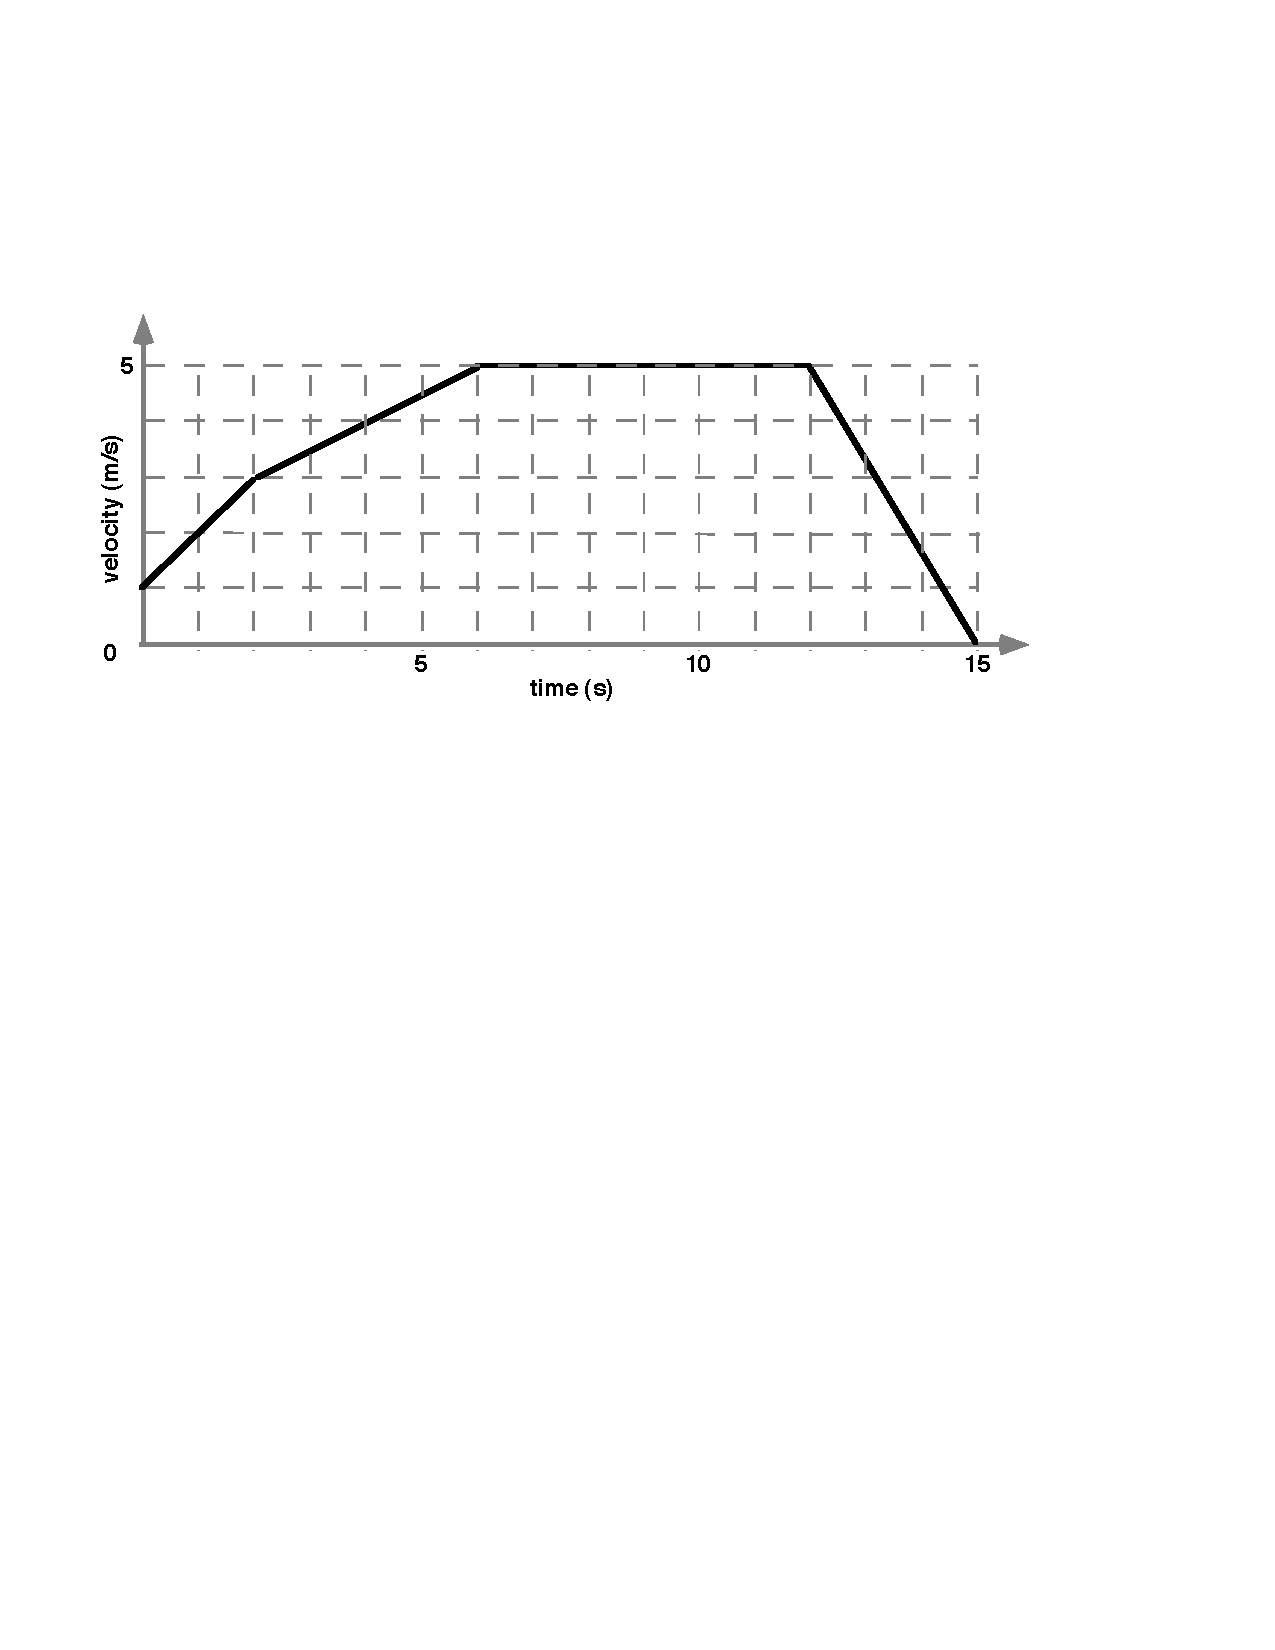
\includegraphics[width=1.0\textwidth]{v_graph.pdf}
        \caption{This graph represents the motion of an object moving in one dimension.
        }
        \label{fig:v}
	\end{center}
        \end{figure}

\begin{enumerate}

\item \textbf{(2 points)}
What is the object's acceleration between $t=3$ and $t=5$ seconds?

\vspace{2cm}

\item \textbf{(2 points)}
How far did the object travel between $t=7$ and $t=11$ seconds?
\vspace{2cm}

\item \textbf{(2 points)}
Indicate on the graph when the object had zero acceleration.

\item \textbf{(2 points)}
What was the object's displacement from $t=10$ to $t=15$ seconds?




\newpage
\item \textbf{(2 points)}
Suppose you read that the force of air resistance is sometimes given by the formula $F_{air}=\rho c A v^2$, where $\rho$ is density in $kilograms/meter^3$, $A$ is area (in $meters^2$), $v$ is speed (in $meters/second$) and F is force (in $Newtons$).  What are the units of the ``drag coefficient" $c$?

\vspace{3cm}


\item \textbf{(2 points)}
For fun, you drop water balloons out of the $3^{rd}$ story window of your apartment (making sure no one is below!).  If you let the balloon go from rest, how far below the window has the balloon fallen after 1 second?

\vspace{2cm}

\item \textbf{(2 points)}
How far has the balloon dropped after 2 seconds?

\vspace{2cm}

\item \textbf{(2 points)}
How far has the balloon dropped after 10 seconds?
   
%\newpage
%\item \textbf{(2 points)}
%Here's some biology:  For warm-blooded animals, metabolic heat production, $E$, scales with the mass, $m$, of an animal, so $E$ is proportional to $m$, or $E\propto m$.  Heat transfer, $Q$,  from an animal to its environment scales with the surface area, $A$, of the animal, so $Q \propto A$.  Finally, most animals are roughly spherical, so their size, $d$, is related to their mass by $d^3 \propto m$, and their surface areas are related to size by $A \propto d^2$.  
%
%Use these claims to explain why large ears are optional on mice, but an elephant without ears would be at a severe disadvantage.  Here's a hint, nearly all of the food energy you eat is given off as body-heat to your surroundings.
\newpage
\item \textbf{(8 points)} Imagine you're in a hot air balloon that's rising at a constant rate of $1m/s$.  At an altitude of $200m$ above the ground, while taking a selfie, your cellphone slips out of your hands and falls to the ground.  How does the motion of the cellphone compare to the motion of the hot air balloon, when plotted by a reference observer on the ground?  
\begin{enumerate}
\item Please sketch two graphs, one altitude vs time, and a second velocity vs time.  
\item Each graph should have a line for the cellphone's motion and a second line for the balloon's motion.  
\item In the velocity graph, label slopes and y-intercepts with numbers.  
\item In the position graph, mark and calculate the time when the cellphone is a maximum altitude.  
\item Take the origin to be $y=0$ at the ground,  and up as the $+y$ direction.
\item use the approximation, $a_y=-10m/s^2$
\end{enumerate}
\newpage


\item
Conventional planting directions suggest that seed potatoes be planted $15$ inches apart, in rows separated by about $3$ feet.  This means that each plant occupies an area of about $0.35~m^2$.  Conservatively, each plant will produce about $2~kg$ of potatoes.  Nutrition labels suggest that a ``large" $369$ gram potato contains about $284$ Calories of food energy.  

I space Kale transplants about $1.5$ feet apart, in rows $24$ inches apart, so each plant takes about $0.28~m^2$ of garden space.  

Before the Irish Potato Famine (which was partially caused by climate change, but mostly caused by government policy and crop mono-culture), Ireland had a large population boom.  Most families flourished on a diet of simply: Potatoes, Kale, and Milk. Potatoes were the main source of energy (calories), Kale provided most of the necessary vitamins, and milk provided fat and protein.  

\begin{enumerate}
\item \textbf{(8 points)} Ignoring the cows, how much garden space does a family of 6 need to raise the kale and potatoes necessary for 8 month of stored food?  Let's assume one kale plant (totally used up) is a day's greens for 3 people. A person engaged in manual labor requires food energy of about $3000~Calories/day$.
\newpage
\item \textbf{(4 points)} At the beginning of the famine, $\approx 1840$, Ireland's population was about 8 million.  About $80\%$ of Ireland is arable (usable for agriculture) and the country's total area is about $70~000~km^2$.  What fraction of the available arable land would be needed to feed the population?
\vspace{6cm}
\item \textbf{(4 points)} The reading earlier this week suggested that, had the export of oats from Ireland been prohibited in the midst of the famine, some starvation could have been avoided, because rather than being exported for sale, food would be locally available.  Based on the land necessary to grow potatoes to feed the population, evaluate this claim.  

Hint: If you want to include a family cow in your analysis, note that it probably requires about an acre of pasture.  If you propagate that estimate out and assume that everyone in Ireland lives in 6-person households, you'd need about $5400~km^2$ of pasture for every family to have a cow.  
\end{enumerate}
\newpage

\item
	One day, my family traveled from Winona to Bloomington MN by car.  While my wife drove, I took occasional odometer/clock readings which are shown in figure \ref{fig:dist}.  The mileage was recorded up to the tenth of a mile, and time was recorded to the nearest minute.  There was no measurement plan, aside from taking a reading every 2-5 minutes. 
	
I started taking distance readings in Winona and we drove to Bloomington by taking 61 up through Kellogg, Wabasha, Lake City, and Red Wing.  At the top of the hill in Red Wing, we cut across to Highway 52, and took 52 North to County 42.  We then took 42 West through Rosemount, and finally took Cedar north to Bloomington.  This wasn't the fastest way, and, however interesting, the described geography isn't necessary to solve this problem.  Using the data in figure \ref{fig:dist}, please answer the following questions:

\begin{enumerate}
\item \textbf{(4 points)} For the whole trip, what was our average speed? 

\item \textbf{(4 points)}While driving, we passed at least 5 Kwik Trip stores.  We stopped at one of them to buy some ``Mike and Ike'' candy.  Based on the data, what was the odometer reading at this stop? 

\item \textbf{(4 points)} During what 10 to 20 minute time period was our average speed greatest? What was this speed?

\item \textbf{(4 points)} At 2:08, our odometer reading was $305.8$.  At 2:07, our odometer reading was $303.9$.  Using the simple average speed formula, $v=\frac{\Delta x}{\Delta t}$, this gives an average speed of $114$ miles per hour.  Were we really driving this fast? Explain.


\end{enumerate}
     \begin{figure}[h]
	\begin{center}
        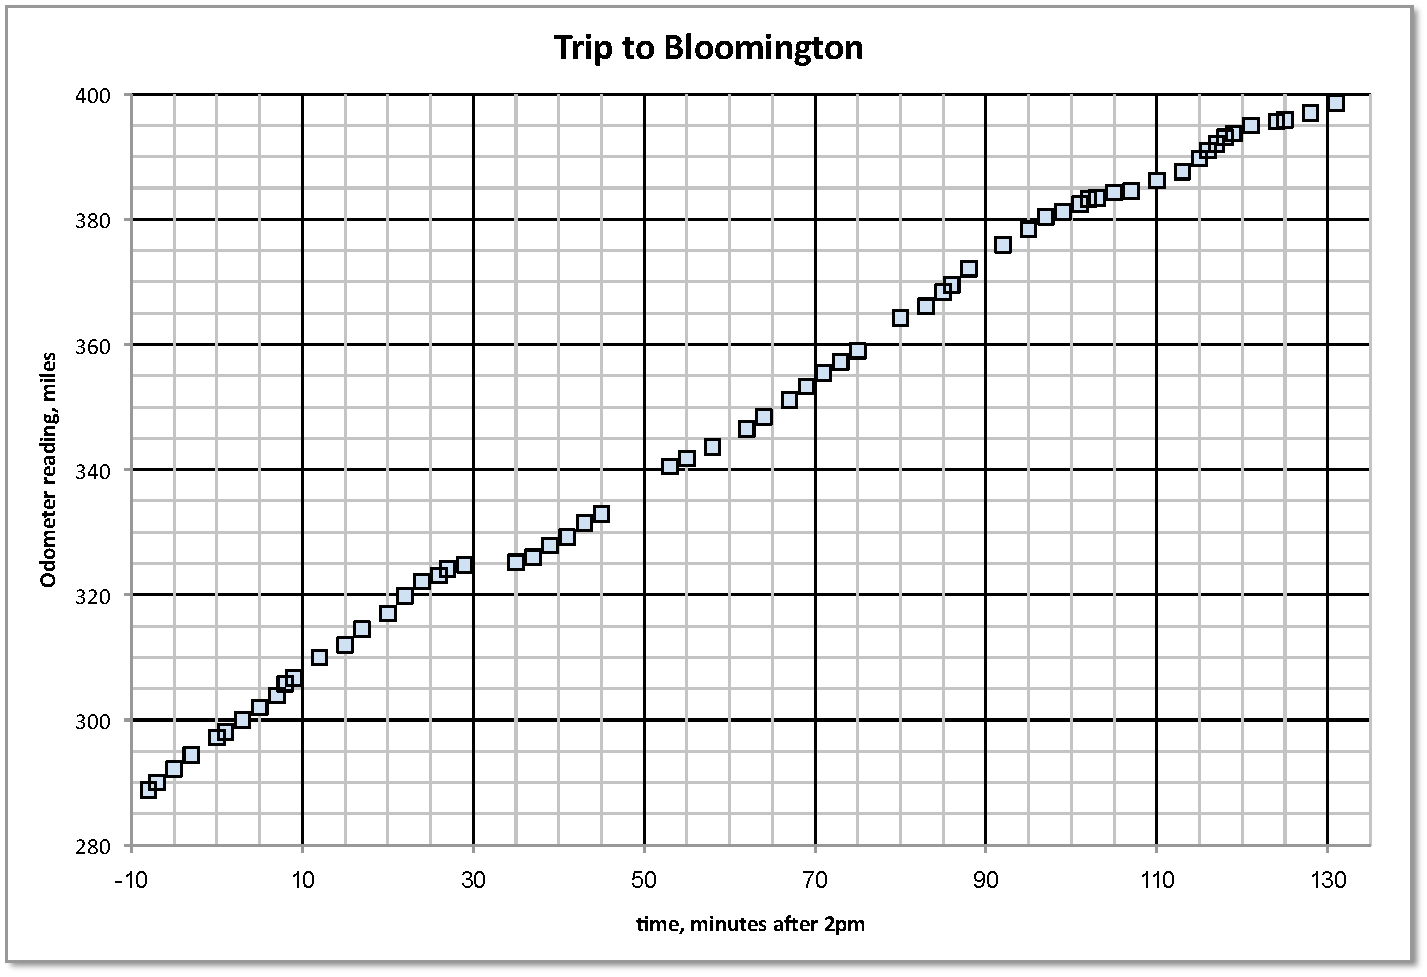
\includegraphics[width=1.2\textwidth, angle=0]{distance.pdf}
        \caption{This figure shows my odometer reading as a function of clock time, as I drove from Winona to Bloomington, MN one friday afternoon.}
        \label{fig:dist}
	\end{center}
        \end{figure}
        
\clearpage

\end{enumerate}
\end{document}